%% edge-neon.tex
\newpage
\subsection{Neon}
\label{paragraph:neon_filter}
\paragraph{Beschreibung des Filters aus Nutzersicht}
Dieses Filter extrahiert Kanten in der aktiven Ebene oder Auswahl und 
umgibt diese mit einem neonartigen Glühen.








\paragraph{Algorithmus} 
%Beschreibung Algorithmus allgemeinsprachlich, 
%Pseudocode, visuell
\begin{algorithm}[h]
\caption{Pseudo-Code des \glqq Neon\grqq-Algorithmus}
\label{algo:neon}
\begin{algorithmic}[1]
\ForAll{$columns \in input$}
	\State lese eine Spalte aus dem Eingabebild
	\ForAll{$pixel \in column$}
		\State berechne neon von oben nach unten
	\EndFor
	\ForAll{$pixel \in column$}
		\State berechne neon von unten nach oben
	\EndFor
	\State merge Ergebnisse in eine Spalte
	\State speichere in Ausgabebild
\EndFor	
\ForAll{$rows \in input$}
	\State lese eine Zeile aus dem Eingabebild
	\ForAll{$pixel \in row$}
		\State berechne neon von links nach rechts
	\EndFor
	\ForAll{$pixel \in row$}
		\State berechne neon von rechts nach links
	\EndFor	
	\State merge Ergebnisse in eine Zeile
	\State \label{neon_datenabhaengigkeit} bilde Gradient von dieser Zeile und einer aus dem Ausgabebild
	\State speichere in Ausgabebild
\EndFor
\end{algorithmic}
\end{algorithm}

Der Algorithmus besteht aus 2 großen Schleifen (detaillierterer Pseudo-Code 
ist in Algorithmus \ref{algo:neon} zu finden).
Beide Suchstufen (in jeder Schleife) erfolgen spalten- bzw. zeilenweise, und zwar von beiden Seiten simultan,
so ist in diesem Fall recht unbeliebte automatische Kachelzerlegung sehr vorteilhaft, da sie Wahrscheinlichkeit dafür erhöht, dass die zum Mergen benötigten Werte noch in Cache zu finden sind.

Für weitere Details siehe Paragraf ``Parallelisierung''.


















\paragraph{Portierung}
\label{neon_portierung}
Der ursprüngliche Code konnte zum größten Teil übernommen werden, natürlich nicht ohne Anpassung der Standardkonstrukte und Schnittstellen.
Auch mehrere unnötige bzw. überflüssige Sprachkonstrukte konnten erkannt und entfernt werden: z.B.  \textcolor{red}{\#radius}.

Des Weiteren wurden im Code viele Variablen umbenannt, was der Qualität und vor allem der Lesbarkeit beitrug, da bevor viele von denen wenigen buchstaben bestanden bzw. aus einer unbekannter Sprache stammen \textcolor{red}{\#k für Head, g für Tail}..

Beachten Sie bitte Hinweise in Paragraf Korrektheit\ref{paragraph:neon_korrektheit}.
















\paragraph{Parallelisierung}
Es gab auch ursprünglich keine funktionale Abhängigkeit zwischen den beiden Stufen (beide äußere For-Schleifen),  jedoch ließ sich der Algorithmus trotzdem nur bedingt parallelisieren. Grund dafür war eine Datenabhängigkeit: In der \ref{neon_datenabhaengigkeit}. Zeile des Algorithmus \ref{algo:neon} werden Ergebnisse der beiden Schritte zusammengeführt. Im sequenziellen Fall hätte es einen guten Grund - bessere Cacheausnutzung - ein der beiden benötigten Felder ist garantiert im Cache (so weit Cache ausreicht) vorhanden.

Wird der Algorithmus parallel ausgeführt, so sollte diese Datenabhängigkeit z.B. durch temporäre Variablen eliminiert werden. 


\subparagraph{Ansätze zur Parallelisierung}
\begin{enumerate}
	\item [] \begin{description} %Platzhalter links
		\item[1) Sections] Der ursprünglich verfolgte Ansatz. Beide äußere Schleifen werden durch ``\#pragma omp sections'' simultan abgearbeitet. Des Weiteren kann auch jede der Schleifen intern parallelisiert werden. Datenabhängigkeit muss eliminiert werden. Siehe Algorithmus \ref{algo:neon_sections}.
		
		Vorteile:
		\begin{itemize}
		\item[\texttt{+}] weniger Datenabhängigkeiten
		\item[\texttt{+}] kritischer Abschnitt ist außerhalb der parallelen Region
		\end{itemize}
		
		Nachteile:
		\begin{itemize}
		\item[\texttt{-}] schlechtere Cache-Ausnutzung
		\item[\texttt{-}] höherer Speicherbedarf (zusätzlicher GeglBuffer nötig)
		\end{itemize}
		

		\item[2) Konservative Schleifenparallelisierung] Unter Annahme, dass die vorhandene Datenabhängigkeit zwecks der besseren Cache-Ausnutzung beibehalten werden soll, muss die erste For-Schleife vollständig abgearbeitet sein, bevor es mit der Zweiten angefangen werden kann (implizite Barriere kann hier gute Dienste leisten). Siehe Algorithmus \ref{algo:neon_conservative}

		Vorteile:
		\begin{itemize}
		\item[\texttt{+}] bessere Cache-Ausnutzung
		\item[\texttt{+}] weniger Eingriffe in den Code
		\end{itemize}
		
		Nachteile:
		\begin{itemize}
		\item[\texttt{-}] kritischer Abschnitt innerhalb der parallelen Region 
		\end{itemize}
	\end{description}
\end{enumerate}

Da GEGL-eigene Methoden zum Lesen und vor allem Schreiben in Ausgabebild als not-thread-safe betrachtet werden und stark gewünscht sind, müssen sie in einem kritischen Bereich geschützt werden.
Der einzige Kritikpunkt an Algorithmus \ref{algo:neon_conservative} besteht darin, dass der kritische Bereich sich in der parallelen Region befindet, was hier zum Flaschenhals resultieren wird - mit zunehmender Threadzahl wird die Effizienz schnell fallen.

Beide Ansätze sind mithilfe von OpenMP realisiert.





\newpage
%PARALLELISIERUNG MIT SECTIONS
\begin{algorithm}[H]
\caption{Pseudo-Code des \glqq Neon\grqq-Algorithmus: Sections}
\label{algo:neon_sections}
\begin{algorithmic}[1]
\State \textcolor{blue}{\#pragma omp parallel sections}\{
\State \textcolor{blue}{\#pragma omp section} 
\ForAll{$columns \in input$}
	\State lese eine Spalte aus dem Eingabebild
	\ForAll{$pixel \in column$}
		\State berechne neon von oben nach unten
	\EndFor
	\ForAll{$pixel \in column$}
		\State berechne neon von unten nach oben
	\EndFor
	\State merge Ergebnisse in eine Spalte
	\State speichere in \textcolor{blue}{temporäres Feld1}
\EndFor	
\State \textcolor{blue}{\#pragma omp section}
\ForAll{$rows \in input$}
	\State lese eine Zeile aus dem Eingabebild
	\ForAll{$pixel \in row$}
		\State berechne neon von links nach rechts
	\EndFor
	\ForAll{$pixel \in row$}
		\State berechne neon von rechts nach links
	\EndFor	
	
		\State merge Ergebnisse in eine Zeile
	\State speichere in \textcolor{blue}{temporäres Feld2}
\EndFor
\State \}
\State \textcolor{blue}{\#pragma omp parallel for }
\ForAll{$pixel \in Ausgabebild$}
	\State \label{neon_keine_datenabhaengigkeit} lese je ein Pixel aus Feld1 und Feld2,  speichere Gradient in Ausgabebild
\EndFor
\end{algorithmic}
\end{algorithm}

%KONSERVATIVE PARALLELISIERUNG
\begin{algorithm}[H]
\caption{Pseudo-Code des \glqq Neon\grqq-Algorithmus: Konservative Schleifenparallelisierung}
\label{algo:neon_conservative}
\begin{algorithmic}[1]
\State \textcolor{blue}{\#pragma omp parallel for }
\ForAll{$columns \in input$}
	\State lese eine Spalte aus dem Eingabebild
	\ForAll{$pixel \in column$}
		\State berechne neon von oben nach unten
	\EndFor
	\ForAll{$pixel \in column$}
		\State berechne neon von unten nach oben
	\EndFor
	\State merge Ergebnisse in eine Spalte
	\State speichere in Ausgabebild
\EndFor	


\State \textcolor{blue}{\#pragma omp parallel for }
\ForAll{$rows \in input$}
	\State lese eine Zeile aus dem Eingabebild
	\ForAll{$pixel \in row$}
		\State berechne neon von links nach rechts
	\EndFor
	\ForAll{$pixel \in row$}
		\State berechne neon von rechts nach links
	\EndFor	
		\State merge Ergebnisse in eine Zeile
	\State bilde Gradient von dieser Zeile und einer aus dem Ausgabebild
	\State speichere in Ausgabebild
\EndFor
\end{algorithmic}
\end{algorithm}








%\begin{figure}
%\centering
%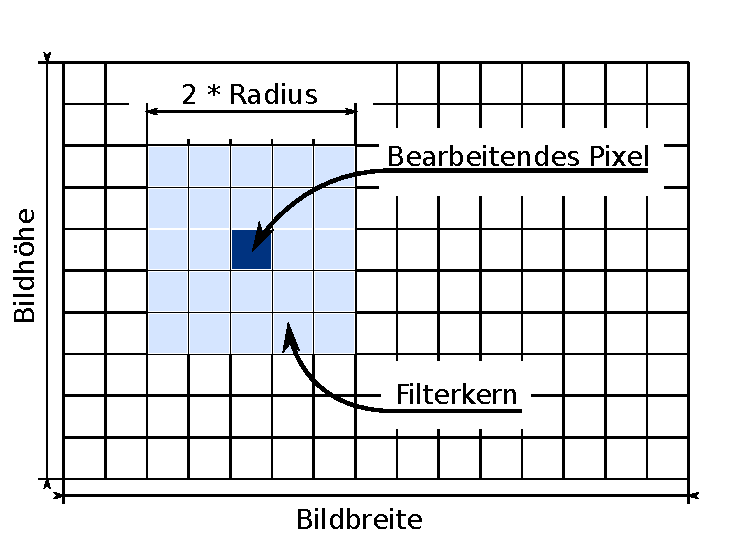
\includegraphics[scale=0.9]{graphs/sgb-grid.pdf}
%\caption{Selective Gaussian Blur. Schematische Darstellung}
%\label{fig:sgb-grid}
%\end{figure} 













